\subsection{Key Continuity Management}
Peter Gutmann in \cite{gutmann-kcm-01} presented key continuity as  mechanism for assuring that the entity with whom a user is currently communicating is the same as the one they were previously communicating with.
Assuming the key resembles the identity of its user, the foundation for key management via key continuity is that once an entity has a remote entity's trustable key, it can validate later the remote entity's identity by confirming that they are still using the same key. The security mechanism relies on how long the key has been in service by its owner. The longer the key is witnessed to have been used, the more it is trusted by other entities. The research also proposed that an external authority manage the key continuity information. A key continuity external authority keeps track of how long a particular key has been used by a specific cryptographic service and responds to inquiries with that information. The document discusses key continuity in several security protocol use cases.
\par
However, the document does not precisely discuss authentication of keys at first use. Rather, the author has mentioned the possibility of users following the \gls{tofu} approach, or out-of-band means, for example, comparing key fingerprints over the phone. Moreover, He did not rule out utilizing digital certificates to verify public keys; nevertheless, he deemed it a more tedious, expensive, and manual process than \gls{tofu}. 

\subsection{Off-the-Record Protocol}
Consider the following scenario: Alice and Bob are alone in a room. Unless they are recorded, no one can hear what they are talking to one other. Therefore, no one knows what they are talking about until Alice and Bob tell them, and no one, not even Alice and Bob, can verify that what they are saying is true. \gls{otr} \cite{otr} aims to achieve the same form of secrecy in the field of instant messaging. The OTR protocol was first released in October 2004 by cryptographers Ian Goldberg and Nikita Borisov. At the time of writing, \gls{otr} is at version 3 \cite{otr3}. \gls{otr} provides a set of essential security features: Encryption, Authentication, Deniability, and forward secrecy.
\par
Abstractly, the protocol flow goes as follows. At first Alice and Bob establish a session encryption key through a \gls{dh} key exchange. Even though each party has established a shared secret, neither has a guarantee about authentication, i.e., no party is sure that the other party is whom it claims to be as a man-in-the-middle attack is possible. Each party owns a long-term public key for identity authentication. These keys are utilized discretely between the communicating parties to prove their identity to each other without sacrificing deniability to third parties. Alice and Bob generate signatures using their long-term private keys, enveloped in messages encrypted using the computed session key. Moreover, HMAC signatures are generated for messages to guarantee integrity as well as authenticity. Alice and Bob generate symmetric signing keys by passing the shared encryption key through hash functions. These signing keys are used to generate HMAC signatures. Next, parties can verify the signature received and consequently have the assurance of the party's identity at the other end of the channel. Assuming there was a man-in-the-middle, he would not be able to forge a signature for either party, and thus, signature verification would fail. Despite the use of digital signatures, they are used within an encrypted channel, and no other party can verify that both parties were communicating. After a message has been received and successfully decrypted, the sender publishes the message signing keys, and both parties delete their encryption keys and start over with the \gls{dh} key exchange to generate a new shared secret. Publishing signing keys enables outsiders to forge messages, enhancing the deniability feature for Alice and Bob. On the other hand, deletion of encryption keys ensures forward secrecy. Lastly, during the exchange of data messages, either Alice or Bob may employ the \gls{smp} \cite{smp} to detect impersonation or man-in-the-middle attacks.

\subsection{SoK: Secure Messaging}
Unger et al. \cite{unger2015sok} presented a comprehensive survey study where they used a methodology they've established to analyze and systematize current secure messaging solutions. Their survey valuably contributes towards an open standard for secure messaging by combining the most promising secure messaging features. The study looks at secure messaging solutions from academic research as well as real-world deployments, which identify innovative and promising ways that have already been implemented but are not covered in academic literature. The presented framework focuses on evaluating three main principles of the surveyed solutions: trust establishment, conversation security, and transport privacy.
For each, they evaluate the security, usability, and ease-of-adoption properties. However, security is the primary aspect relevant to our work.
\par
Trust establishment is defined as the procedure through which users ensure that they are communicating with the intended parties, i.e., a combination of long-term key exchange and long-term key authentication. While, transport privacy is concerned with preserving the privacy of users by obscuring metadata of messages during transit, such as the sender, receiver, and which conversation the message belongs to. Nevertheless, the aspect most relevant to our work is conversation security. It relates to protecting messages' security and privacy; and comprises the methods used to encrypt communications, the associated data, and the cryptographic algorithms employed. In addition to confidentiality, authentication, and integrity, discussed earlier, below are additional security properties. The following properties are relevant to two-party communication only as group communication is out of our scope.
\begin{itemize}
	\item \textit{Participant Consistency:} When one honest party accepts a message, all other honest parties are assured to have the same view of the participant list.
	
	\item \textit{Destination Validation:} When an honest party accepts a message, they may verify that they were included in the message's intended recipients list.

	\item \textit{Anonymity Preserving:} The underlying transport privacy architecture's anonymity characteristics are not jeopardized by the message exchange protocol.
	
	\item \textit{Speaker Consistency:} The order of messages transmitted by each participant is agreed upon by all participants. During the protocol, or after each message is transmitted, a protocol may execute consistency checks on blocks of messages.

	\item \textit{Causality Preserving:} It is possible to prevent showing a message before messages that are causally related to it in the implementation.
	
	\item \textit{Global Transcript:} All of the messages are displayed in the same order to all of the participants. It's worth noting that this presupposes speaker consistency.
	
	\item \textit{Deniability:} In some secure communications protocol use cases, deniability is a desired property. It refers to the inability of others to verify that a particular individual transmitted the data. However, if Bob receives a message from Alice, he can be confident that Alice sent it, but he cannot prove it to anybody else. Anyone can forge messages after a conversation to make them look like they came from them. However, if it is during a conversation, participants can rest assured that the messages they exchange are authentic and have not been modified by an intruder. Secure messaging protocols that offer deniability can assure the user that anyone can forge messages on their behalf after a conversation has ended, but not during a conversation. Deniability may be realized by conversation security protocols in a variety of forms. The authors define the following deniability-related features.
	
	\begin{itemize}
		\item \textit{Message Unlinkability:} If a judge believes a participant authored one message in a conversation, that does not mean they authored all of the messages.
		
		\item \textit{Message Repudiation:} Under the assumption that the judge does not have access to the accused participant's long-term secret keys, provided a conversation transcript, and all cryptographic keys, including session keys, there is no proof that any individual user authored a given message.
		
		\item \textit{Participation Repudiation:} There is no proof that the honest participant was in a conversation with any of the other participants, given the conversation transcript and all cryptographic key material for all but one accused participant.
		
	\end{itemize}
	\item \textit{Forward} and \textit{Future secrecy} are discussed later in chapter \ref{ch:postcomp}
\end{itemize}
Their study concluded a number of outcomes.
First, the usability and adoption of trust establishment solutions with solid security and privacy guarantees are low. However, other hybrid approaches that have not been thoroughly examined in the academic literature may give better trade-offs in reality.
Second, most of the stated conversation security properties are not mutually exclusive; nonetheless, combining protocol designs has considerable potential for improvement. For two-party conversation security, the most outstanding and promising solution of the bunch was the per-message ratcheting with resilience for out-of-order messages combined with deniable key exchange protocols, as implemented in Axolotl (now called the double ratchet algorithm), can be employed today at the cost of additional implementation complexity with no significant impact on user experience. 
Finally, transport privacy remains a challenging problem as it is difficult to solve without paying significant performance penalties. Among the analyzed solutions, no suggested approaches provided strong transport privacy properties against global adversaries while also remaining practical.

%	\item immediate decryption:
%		the fact that messages might arrive out of order or be lost entirely. Additionally, parties can be offline for extended periods of time and send and receive messages asynchronously. Given these inherent constraints, immediate decryption is a very attractive feature. Informally, it ensures that when a legitimate message is (eventually) delivered to the recipient, the recipient can not only immediately decrypt the message but is also able to place it in the correct spot in relation to the other messages already received. Furthermore, immediate decryption also ensures an even 	more critical liveness property, termed message-loss resilience (MLR) in this work: if a message is permanently lost by the network, parties should still be able to communicate
\subsection{The TESLA Broadcast Authentication Protocol}\label{bg:tesla}
Source authentication and integrity are among the most challenging aspects of protecting broadcast communication. In other words, receivers of broadcast data can verify that the received data originates from the claimed source and the data has not been modified en route. This difficulty is exacerbated by mutually untrustworthy receivers and unreliable communication settings in which the sender does not retransmit dropped packets. While many broadcast networks can effectively convey data to several recipients, they also make it easy for a malicious user to impersonate the sender and insert broadcast packets. This is known as a packet injection attack. Participants must use a broadcast authentication protocol to resist the attack, allowing receivers to verify that the alleged sender indeed transmitted the received packet. Nevertheless, using asymmetric cryptography to sign each message is a high overhead for time and bandwidth. Similarly, simply using \glspl{mac} does not solve the problem as any receiver with the shared secret can impersonate the sender and forge data.
\par
Perrig et al. \cite{perrig2003tesla} aimed to tackle the problem by proposing the \gls{tesla} protocol. \gls{tesla} inflicts low overhead for communication and computation while generating and verifying authentic information. Moreover, it is scalable to large numbers of receivers and tolerates packet loss. Nevertheless, \gls{tesla} requires the sender and the receivers to be at least loosely time-synchronized as well as the receiver or the sender is required to buffer some messages. Loosely time synchronization is that a receiver does not need to know the difference between the sender and the receiver’s time, however, it is only interested in an upper bound on the sender's time, or also know as the maximum time synchronization error. \gls{tesla} also relies on one-way chains which are repeated use of one-way hash functions. Similar in principle to KDF chains explained in section \ref{backgroung:kdf}. 
\par
In principle, the sender in \gls{tesla} generates a chain from an initial random secret key $s_\ell$ by iteratively applying the one-way hash function till the desired chain length is achieved. All intermediate keys generated are stored securely as well as the final key $s_0$. The final key is referred to as the commitment key. The sender divides the timeline into intervals while assigning each key to an interval. A key is used to generate \glspl{mac} for the messages sent during the specified time interval. However, keys are used in an opposite order to how they were generated, as depicted in figure \ref{fig:tesla}. During an interval, the sender uses the key to generate \glspl{mac} but key remains secret to the sender through out that interval. Meaning that receivers are unable to verify the \gls{mac} during that interval and also no malicious entity is able to forge a valid message. After the interval has passed, the sender publishes the now expired key for receiver to verify messages whose \gls{mac} was generated using that key. Receivers also verify the correctness of the disclosed key by inputting it into the one-way chain. If after a number of iterations the commitment key is reached $s_0$, then the key belongs to the expected chain and is valid.
\begin{figure}[hptb]
	\centering
	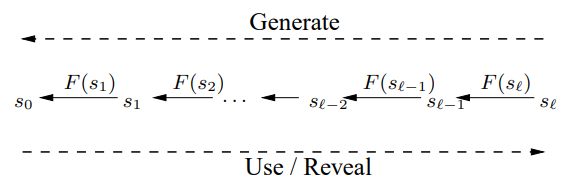
\includegraphics[scale=0.65]{Images/tesla.png}
	\caption{\gls{tesla} keys generation and usage \cite{perrig2003tesla}.}
	\label{fig:tesla}
\end{figure}
\par
Nevertheless, before authenticating messages with \gls{tesla} a receiver must be loosely time synchronized with
the sender, know the disclosure schedule of keys, and receive an authenticated key of the one-way key chain. The required information can be authentically obtained via digitally signed broadcast message, or over unicast with each receiver.
\par
Despite the security guarantees of the innovative approach, \gls{tesla} might not be suitable for some use cases due to the following limitations.
\begin{itemize}
	\item There is an initialization phase in which the first element of the hash chain must be transmitted to all recipients. In this step, authentication is accomplished using standard asymmetric cryptography. Furthermore, a new chain must be formed once the hash chain is depleted.
	\item The verification of a message or a set of messages is only possible once the next is received.
\end{itemize}

\subsection{A Survey of Key Bootstrapping Protocols}
Malik et al. \cite{bs-survey} provide a comprehensive survey study for a set of well-developed bootstrapping protocols in the context of \gls{iot}. They discuss the role of security and, in particular, key bootstrapping protocols at different layers of the \gls{iot} architecture. Next, they suggest a taxonomy for classifying key bootstrapping protocols, as shown in figure \ref{fig:bs-taxonomy}. The considered protocols are classified under the mentioned taxonomy and analyzed with the focus primarily on bootstrapping protocols based on asymmetric key distribution schemes. Lastly, they compare the surveyed key management schemes based on security and functionality features: Mutual Authentication, Forward Secrecy, resilience to key compromise impersonation, and resilience to replay attacks.
\begin{figure}[hptb]
	\centering
	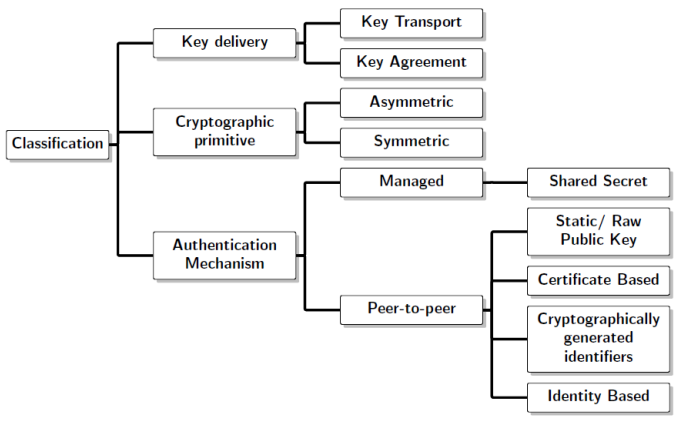
\includegraphics[scale=0.5]{Images/taxonomy.png}
	\caption{Taxonomy for classifying bootstrapping protocols \cite{bs-survey}.}
	\label{fig:bs-taxonomy}
\end{figure}

%\subsection{On post-compromise security}
%study post-compromise security in (classic) key exchange. Here, security shall be achieved even for sessions established after a full compromise of user secrets. This necessarily requires mixing user state information with key material that is newly established via asymmetric techniques, and is thus related to RKE.